\documentclass[conference,letterpaper,onecolumn,11pt]{IEEEtran}

%\renewcommand{\rmdefault}{ptm}
%\usepackage[scaled=0.92]{helvet}
%\usepackage{courier}
%\normalfont % in case the EC fonts aren't available
%\usepackage[T1]{fontenc}
%\parskip=2pt\parindent 0pt

\usepackage{graphicx}
\usepackage{psfrag}
\usepackage{stfloats}
\usepackage{epsfig}
\usepackage{pifont}
\usepackage{amssymb}
\usepackage{fixltx2e}
\usepackage{amsmath}
\usepackage{rotate}
\usepackage{anysize}
\usepackage{float}
\usepackage{fancybox}
\usepackage{subfig}
\usepackage{setspace}

\newcommand{\pig}[1]{\mbox{\boldmath ${#1}$}	}

\newtheorem{Theod}{{\bf Definition}}

\def\boldtild{\mathaccent"0365 }
\newcommand{\puttilde}[1]{\boldtild{\boldmath #1}}

\setlength{\oddsidemargin}{5mm}
\setlength{\evensidemargin}{5mm}
\setlength{\topmargin}{4mm}
\setlength{\textwidth}{15cm}
\setlength{\columnsep}{5mm}
\setlength{\textheight}{24cm}

\doublespacing
\begin{document}

\title{Symbolic Analysis and Reordering of Nonlinear Circuit's equations in order to Accelerate Homotopy Simulation}

\author{\authorblockN{H\'ector V\'azquez-Leal}
\authorblockA{Universidad Veracruzana\\
Facultad de Instrumentaci\'on Electr\'onica\\
Xalapa, Veracruz, M\'exico\\
Email: hvazquez@uv.mx}
\and
\authorblockN{Arturo Sarmiento-Reyes}
\authorblockA{INAOE\\
Departamento de Electr\'onica
}
\and
\authorblockN{Luis Hern\'andez-Mart\'{\i}nez}
\authorblockA{INAOE\\
Departamento de Electr\'onica
}
\and
\authorblockN{Roberto Casta\~neda-Sheissa and Jes\'us S\'anchez-Orea}
\authorblockA{Universidad Veracruzana\\
Facultad de Instrumentaci\'on Electr\'onica\\
Xalapa, Veracruz, M\'exico\\
}
}

\begin{singlespace}
\maketitle
\end{singlespace}

\begin{abstract}
In this work a symbolic study will be performed to establish the non-linearity degree of nodal equations result of the MNA analysis performed in non-linear circuits. The goal is to provide a reordering criterion for nodal equations that, eventually, accelerate the Homotopy simulation. A criterion will be formulated to rate non-linearities, allowing to numerically set a level of no-linearity to nodal equations so, afterwards, equations will be reordered in several Homotopy simulations of a non-linear circuit.
\end{abstract}

\section{Introduction}

Electronics is a highly competitive industry, where the consumer market pressures produce a technological race that includes aspects like: portability, low energy consumption, and increase in features and functionalities. An example of this technological race are cellular phones. This devices, originally,  were bulky and heavy, useful just to make phone calls; nowadays, cellular phones are light, small and includes functionalities like: radio and television tuner, video games, sophisticated computer programs, among others. Besides, cellphones have absorbed products like: electronic agendas, alarms, beeper, to name a few, that used be sold separately. All of this have been possible by new manufacturing processes, which makes possible place more transistors in the same silicon area. Therefore, the integration of so many transistors in an integrated circuit (IC) has increased the circuit complexity. Thus, when the IC is designed it is often to work with so many different design blocks (digital, analog, high speed serial interfaces, FR, microwave circuits) according to the new features to be included in the new product.

What has been mentioned above translates in an increase of dimensions and complexity for the equilibrium equation resulting of the DC analysis of the circuit, generating the need of new and better numerical tools that allows to locate one or more operating points. In this context, Homotopy methods \cite{stat_1} have been recently used in the task to find the operating point for non-linear resistive circuits, when the equilibrium equation has a solution difficult to find, or when the circuit has more than one solution. To analyze any circuit it is necessary to establish, first, the equilibrium equation for the system.

The Newton-Raphson (NR) method is employed in most of the integrated circuit simulators. The reason for the widely use of the NR method is because the convergence rate is quadratic \cite{cont_quasi}, minimizing computing times in simulations. Nevertheless, the NR method is prone to certain convergence problems [43] like: oscillation and divergence. Such convergence problem is specially noticeable in electronics where non-linear equations system from complex circuits are solved, these complex circuits combine blocks like: digital, analog, high-speed digital interfaces, RF, microwave circuits, among others. Therefore, it is necessary to develop backup methods or replacements for the NR method. Besides, circuit designers have to deal with convergence failures on the NR method and backup methods, so, as a last resort, they modify some parameters within the numerical engine expecting to achieve convergence. This situation increase design times making it more expensive and slows down the entire design process, affecting competitiveness in the end. This situation by itself justifies the use of alternate methods to NR, like Homotopy to locate the operating point. Nevertheless, there are more reasons to use Homotopy methods, like the existence of multiple operating points. Unlike NR method, Homotopy \cite{netwth_lasr,homo_iscas05,homo_ArtificialP} is capable to locate multiple operating points. This is very important since there is a chance that designer approves a DC operating point (found by the NR method) but other operating point (it is possible for the circuit to have more than one operating point) is physically present in the circuit. This translates in circuit malfunctioning and costly consequences for the company.

Homotopy methods \cite{cont_bra,cont_kao,cont_chu1,cont_leu11,cont_ritch} have demonstrated being useful to locate multiple operating points and converge to solutions when the NR method is unable to. Nevertheless, the Homotopy methods have the drawback of being slow, compared to the speed of the NR method.

On this work, the modified nodal analysis \cite{mnaxx,stat_1} (MNA) is employed to establish the equilibrium equation for the circuit.

In its general form, the equilibrium equation for non-linear resistive circuits has the form:

\begin{equation}
\pig{f}(\pig{x})=\pig{0}
\label{Fequilibrio3}
\end{equation}

where $\pig{f}$ is a system with $n$ non-linear algebraic equations and $\pig{x}$ is the unknowns vector of the system. When the MNA is employed, $\pig{x}$ is the vector that contains nodal voltages and currents for the NA compatible elements \cite{Schwa_book}.

Once obtained the equation (\ref{Fequilibrio3}), proceed to establish the Homotopy equation, which has the general form:

\begin{equation}
\pig{H}(\pig{f}(\pig{x}),\lambda )=0
\label{homotopia3}
\end{equation}

where $\lambda$ represents the Homotopy parameter.

\section{Reordering}

One possible way to decrease computing time in Homotopy simulations is by swapping equation\'s setup. Therefore, in order to illustrate the effect of the ordering has in the Homotopy formulation, a very simple example of a circuit is analyzed next applying Chao's Homotopy scheme \cite{cont_kao}. In this method, the Homotopy equation is given by:

\begin{equation}
{ {{d f_i[\pig{x}(p)]} \over{dp}} + f_i[\pig{x}(p)]=0}
\label{chao}
\end{equation}
con $f_i(\pig{x}(0))=0$ para $i=1,2,\ldots,n-1$.

The $n$-th equation is:

\begin{equation}
{  {{d f_n [\pig{x}(p)]} \over {dp} } \pm f_n [\pig{x}(p)]=0}
\label{chao2}
\end{equation}

where the sign change for the $n$-th equation, $f_n$, should occur at points where Jacobian sign changes (the goal is to avoid moving away from solutions path) and at solutions (to continue the inspection for more solutions).

This method consists in finding one solutions path, which coincides with the intersection of the ($n-1$) surfaces defined by $\pig{f}_i=\pig{0}$, $i=1, 2, \ldots, n-1$. In such a way that Homotopy path is traced on the plane for the $n$-th equation.

The behavior for the above Homotopy strongly depends on equation (\ref{chao2}), due to sign change, i.e. the continuation procedure is linked exclusively to the $n$-th equation. Nevertheless, when equilibrium equation is established by MNA, the $n$-th equation {\bf will always} corresponds to the branch relationship for any non-NA compatible element present in the circuit.

\begin{figure}[t]
\centerline{
\epsfxsize=70mm
\epsffile{chap3/figs/erdd.eps}}
\caption{Circuit with three solutions.}
\label{cirejemplo}
\end{figure}

To show how equations order affect the formulation for the equilibrium equation, the circuit shown in figure (\ref{cirejemplo}) will be used; it has linear conductance ({$K_a$}), a diode ({$K_b$}) with exponential branch function, and a non-linear conductance ($K_c$) with polynomial branch function. Applying the MNA method the obtained system is:

{%\tiny
\begin{equation}
\left[ \begin{array}{cccc}
K_a  & -K_a & 0 & +1\\
-K_a & K_a  & 0 & 0 \\
0   & 0    & 0 & 0 \\
+1   & 0    & 0 & 0 
\end{array} \right]
\left[ \begin{array}{c}
v_1\\ v_2\\ v_3\\ i_{V_1}
\end{array} \right]
+ \newline \\
\left[ \begin{array}{c}
0\\ i_{K_b}\\-i_{K_b}+i_{K_c} \\ 0 \end{array} \right]
-
\left[ \begin{array}{c}
0\\ 0\\ 0\\V_1 \end{array} \right]
= \pig{0}
\label{eqsimple}
\end{equation}}

where $v_1$, $v_2$, and $v_3$ are nodal voltages, $i_{V_1}$ is the current for the independent voltage source, and currents $i_{K_b}$ and $i_{K_c}$ are the ones flowing through non-linear conductances $K_b$ and $K_c$, respectively. The fourth equation corresponds to branch relationship for the independent voltage source:

\begin{displaymath}
v_1-V_1=0
\end{displaymath}

This equation is linear, which can be solved in the first iteration, regardless of the numerical method employed to trace the Homotopy path, such that nodal voltage $v_1$ is subject of the independent voltage source $V_1$. Hence, is not useful place at the end during the Homotopy simulation. So, it would be inconvenient linking the continuation process to an $n$-th equation whose branch relationship is non-linear.

Figure (\ref{rutas}) shows the geometric solution of the non-linear algebraic equations system (\ref{eqsimple}). Three planes can be note in the figure:

\begin{itemize}
\item  Exponential plane $S_1$ with the diode characteristics $K_b$.
\item  Polynomial plane $S_2$ with characteristics of the non-linear conductance $K_c$.
\item  "Load" plane $S_3$, which combines voltage source equation $V_1$ with characteristics of the linear conductance $K_a$.
\end{itemize}

Solutions for the equations system are noted by white points at intersection of the planes and represent the DC operating points for the circuit in figure (\ref{cirejemplo}).

\begin{figure}[!h]
\centerline{
\epsfxsize=70mm
\epsffile{chap3/figs/p3.eps}}
\caption{Homotopy paths linked to equilibrium equation for the circuit in figure  (\ref{cirejemplo}).}
\label{rutas}
\end{figure}

For the previous circuit there are three Homotopy paths:

\begin{itemize}
\item $P_a$, this path lays on the oblique plane.
\item $P_b$, this path lays on the exponential plane.
\item $P_c$, this path lays on the polynomial plane.
\end{itemize}

Each path ($P_a,P_b$ and $P_c$) match the election of a $n$-th different equation, which represents different Homotopy paths. Thus, the $n$-th function ($f_n(\pig{x})$) should be selected using the appropriate criterion to calculate the non-linearity level for each $f_i(\pig{x})$.

\section{Branch functions classification}
\label{cfr}

In order to classify the nodal equations by its non-linearity degree, it is necessary, first, classify the branch functions for non-linear elements by their non-linearity degree since these elements provide currents that flow to the nodes and, therefore, determine the non-linearity degree for the nodal equation related to the node.

Given the modified nodal analysis applied to formulate the equilibrium equation, based on the Kirchhoff current law, it is possible to establish:

\begin{Theod}
The sum for all currents coming in and out of a given node equals to zero.
\end{Theod}

Therefore, it is possible to infer the level of non-linearity for a nodal equation, measuring the non-linearity level of branch functions for each element connected to the node under analysis.

To perform the analysis for the type of branch functions, these are classified as:

\begin{itemize}
\item {\bf Linear function}\hfill \par
Those functions that comply with the homogeneity and superposition principles. The static elements that comply with these principles are resistors and linear conductances \cite{Vlach_book}, their branch characteristics are given by:

\begin{displaymath}
u= R i \qquad \mbox{y} \qquad i=G u
\end{displaymath}

respectively, where $R$ and $G$ are values for resistance and conductance.Linear functions will be assigned weight of 0.

\item {\bf Non-linear function}\hfill \par
Those functions, contrary to linear functions, that {\bf do not} comply with the homogeneity and superposition principles. To classify non-linear branch functions, this work resorts to the classification provided by \cite{cont_leu11}. In this work, non-linear branch functions are initially classified as:

\begin{dinglist}{226}
\item Weakly non-linear functions
\item Strongly non-linear functions
\end{dinglist}
\end{itemize}

\subsection{Weakly non-linear functions}
Weakly non-linear are classified as follows:

\begin{itemize}
\item {\bf Non-bounded}\hfill\par
	This classification is also subdivided into:
      \begin{itemize}
      \item Type $U^+$\hfill \par
	if $f(x)\to \infty$ when $x\to \infty$,
            and $f(x)\to -\infty$ when $x\to -\infty$
      \item Type $U^-$\hfill \par
	if $f(x)\to \infty$ when $x\to -\infty$,
            and $f(x)\to -\infty$ when $x\to \infty$      
      \end{itemize}
 
      Figure (\ref{UB}) shows both kinds of non-bounded functions.
      \begin{figure}[!h]
       \centerline{
       \epsfxsize=80mm
       \epsffile{chap3/figs/Ub.eps}}
       \caption{Non-bounded functions.}
       \label{UB}
      \end{figure}
      
\item {\bf Semi-bounded}\hfill\par
	 This classification is subdivided as:
      \begin{itemize}
      \item Type $H^+$ \hfill \par
        if $f(x)\to \infty$ when $x\to \infty$,
        and $|f(x)|$ remains bounded  according to $x\to -\infty$
      \item Type $H^-$\hfill\par
            if $f(x)\to -\infty$ when $x\to -\infty$,
            and $|f(x)|$ remains bounden according to $x\to \infty$
      \end{itemize} 
      
   Figure (\ref{HB}) shows both kinds for semi-bounded functions.
      \begin{figure}[!h]
       \centerline{
       \epsfxsize=80mm
       \epsffile{chap3/figs/Hb.eps}}
       \caption{Semi-bounded functions.}
       \label{HB}
      \end{figure}


\item {\bf Double-bounded functions}\hfill\par
      \begin{itemize}
      \item Type $B$\hfill\par
        if $|f(x)|$ remains bounded according to $|x|\to \infty$
      \end{itemize}

	  Figure (\ref{fig:subfig:BB}) shows a double-bounded function.  

\begin{figure}[hbtp]
\begin{center}
%% --- start of first subfigure ---
\subfloat[Double bounded function.]{
	\label{fig:subfig:BB}
	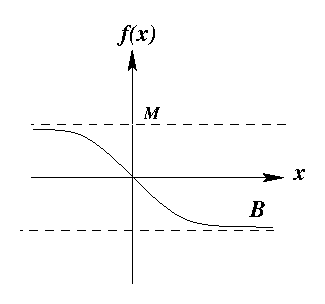
\includegraphics[scale=0.8]{chap3/figs/bb.eps}}
\hspace{0.4in}
%% --- start of second subfigure ---
\subfloat[Non-linear strong function.]{
	\label{fig:subfig:nl}
	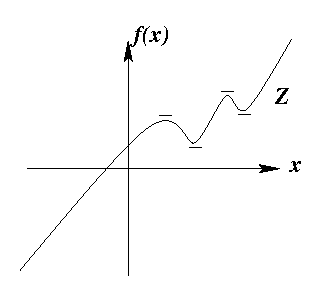
\includegraphics[scale=0.8]{chap3/figs/nl.eps}}
\end{center}
\caption{Non-linear branch functions.}
\label{fig:subfig}
\end{figure}      
\end{itemize}

\subsection{Strongly non-linear functions}

{\bf Strongly} non-linear branch functions are weighed by the number of local maximums and minimums. In such a way that the greater number of maximums and minimums the greater level of non-linearity. Figure (\ref{fig:subfig:nl}) shows an example of strongly non-linear function.

\section{Weight assignment for non-linear branches}

It has been showed a classification for non-linear branch functions, so it is now possible to assign weights to every type of non-linear function. Table (\ref{PesoRamas}) shows assigned weights to weak non-linear branch functions. Lower weight is assigned to branch functions of type non-bounded ($U^{\pm}$) because these do not have asymptotes and their behavior is reminiscent to a resistor or linear conductance. For branch functions of type semi-bounded higher weight is assigned because they have one asymptote. Finally, the highest branch weight is for branch function of type $B$ because it has two asymptotes. The weight calculation for the strongly non-linear functions is achieved by the application of the following simple formula:

\begin{displaymath}
\beta=Z+3
\end{displaymath}

where $Z$ is the number of local maximums and minimums, Fig. \ref{fig:subfig}.

\begin{table}[!h]
\center{
\begin{tabular}{||c|c||}
\hline\hline
Types  & Weight $W$ \\ \hline\hline
$U^{\pm}$ &  1 \\ \hline
$H^{\pm}$ & 2 \\ \hline
$B$ & 3 \\ \hline \hline
\end{tabular}
}
\caption{Weight for weakly non-linear functions}
\label{PesoRamas}
\end{table}

For the case $Z=0$, it has been determined that branch of type weak non-linear. Then, the minimum value for $Z$ is 1, so the weight for a strong non-linear branch is 4, then it will always be heavier than the double-bounded non-linear function ($B$).

\section{Weigh criterion for Nodal Equations}

In the previous section was explained how equations originated by the MNA method for non-linear circuits affect Homotopy paths, because the non-linearity level is different for each equation. Therefore, it is important to weigh equations based on their non-linearity level. Besides, the first step for weighing nodal equations has been already taken by showing a classification of non-linear branch functions. Starting from this classification it is possible to establish a weigh criterion for nodal equations.

Two basic criteria have been elaborated (\cite{homo_SMACD,homo_ICECS}) for weigh nodal equations, these are: non-linear incidence level criterion and non-linear incident type criterion.

Both criteria is described next:

\begin{description}
\item {\bf Number of non-linear resistors incidence level criterion}\hfill\par

This criterion is based on determining the number of incident non-linear components, to each node, considering this number as the weight for the nodal equation related to the node. By applying this criterion, turns out that in figure (\ref{rams}) the node with higher non-linearity is node ({\sf b}) because it has the higher number of incident non-linear branches.

\begin{figure}[!h]
\centerline{
\epsfxsize=120mm
\epsffile{chap3/figs/twonodes.eps}}
\caption{Non-linearities connected to nodes.}
\label{rams}
\end{figure}

This weigh criterion can be summarized by the following formula:

\begin{equation}
\puttilde{\delta}_i =  \mbox{\# incident non-linear elements}
\end{equation}

where $\puttilde{\delta}_i$ is the incidence non-linear level for the $i$-th node.

\item {\bf Incident non-linear type criterion}\hfill\par

The prior criterion could lead to wrong considerations, because it does not take into account the types of non-linearities of the incident branches into nodes. For instance, a node could have the lowest number of incident non-linear elements and still have associated the highest non-linear nodal function. Therefore, a second criterion has been created, which is based on the assignment an specific weight for every node (nodal equation) depending on the type of non-linearities incident to it. So, the wight of a node is equal to the sum of weights of branch functions for all non-linear elements incidents to the node. This weigh criterion can be summarized by the following formula:

\begin{equation}
\puttilde{\zeta}_i = \Sigma (\mbox{weight of incident non-linearities})
\end{equation}

where $\puttilde{\zeta}_i$ is the sum of weights of incident non-linearities to the $i$-th node. An example can be seen in Fig. \ref{rams}, at node (a).
\end{description}

\section{Transactor treatment}

Branch constitutive functions have been considered so far, these involve variables (voltage and current) for the same branch, i.e. elements that depend in variables from another branch have not been considered, like branch functions for linear transactors or controlled sources. Linear transactors are part of models for several devices among which are bipolar transistors, field effect transistors, operational amplifiers, etc., so they have practical importance. Even though transactors are linear, there might be the case that the controlling variable comes from a non-linear element, which cause that non-linearity be {\em inherited} \cite{homo_ECCTD} by the transactor and the output branch of it is handling a non-linear variable. Such is the case for the large-signal Ebers-Moll model for the bipolar transistor \cite{misc_getr}, where the linear transactor is controlled by the current flowing through a non-linear conductance, such that the transactor handles a non-linear current at the output. As a result of this situation, the effects of linear transactors should be taken into account in the weigh criterion when the controlling variable comes from a non-linear element, as shown in the scheme in figure (\ref{depX}).

Depending in whether the output variable of the transactor is current or voltage, the equilibrium equation will be affected; either in the corresponding nodal equation or the non-NA branch relationship, as shown in figure (\ref{depY}). In transactors with current as output variable, this is seen as a non-linear current flowing to the node, while for transactors with voltage as output variable, these involve a non-NA compatible equation.

\begin{figure}[!h]
\psfrag{expre1}{\scriptsize{$EV_1 = \puttilde{f}(EV_2)$}}
\psfrag{ivar}{\scriptsize{$\puttilde{\pig{\i}}$}}
\psfrag{vvar}{\scriptsize{$\puttilde{\pig{u}}$}}
\psfrag{exprea}{\small{$EV_{out} = \alpha \tilde{\i}$}}
\psfrag{expreb}{\small{$EV_{out} = \alpha \puttilde{u}$}}
\centerline{
\epsfxsize=70mm
\epsffile{chap3/figs/ivdep.eps}
}
\caption{Linear transactors involving non-linear variables.}
\label{depX}
\end{figure}

\begin{figure}[!h]
\psfrag{outI}{\scriptsize{$\pig{i}_o = \alpha \puttilde{EV}$}}
\psfrag{outU}{\scriptsize{$\pig{u}_o = \alpha \puttilde{EV}$}}
\psfrag{ix}{\scriptsize{$\puttilde{\pig{i}}_o$}}
\psfrag{vx}{\scriptsize{$\puttilde{\pig{u}}_o$}}
\centerline{
\epsfxsize=120mm
\epsffile{chap3/figs/both.eps}
}
\caption{Output variables for transactors affecting equilibrium equation.}
\label{depY}
\end{figure}

According to the weight assignment criterion, the weight for non-linear elements $\rho$ is inherited to the transactors multiplied by coupling factor $\alpha$, which is expressed as $\alpha\rho$.

\section{Study of non-NA compatible elements}

When the MNA method is employed to establish the equilibrium equation, given in equation \ref{Fequilibrio3}, it has the general form:

\begin{displaymath}
\pig{f}(\pig{x})=
\left[\begin{array}{c}
f_1(\pig{x}) \\ \vdots\\ f_j(\pig{x}) \\ \vdots\\ f_n (\pig{x})
\\\hline
r_1(\pig{x}) \\ \vdots\\ r_k(\pig{x}) \\ \vdots\\ r_m (\pig{x})
\end{array} \right]
= \pig{0}
\end{displaymath}

where $f_j(\pig{x})=0$ is nodal equation for the $j$-th node and $r_k(\pig{x})=0$ is branch equation for the $k$-th non-NA compatible element. There are $n$ nodes and $m$ branch functions from the non-NA compatible elements. Therefore, the task to assign weights to the equations from the MNA method still is not finished because, at this moment, there have been weighed $n$ nodal equations, remaining to assign wights for $m$ equations introduced by the non-NA compatible elements. Since non-NA elements contribute with additional functions, it is only necessary to assign the weight of the branch function for the $m$-th element according to the classification for the non-linear functions $u$-$i$.

\section{Weight assignment procedure}

In this section the concepts exposed in previous sections will be summarized and the procedure to automate the process of weight assignment to nodal equations will be carried out. The weigh procedure can be resumed in the following steps:

\begin{enumerate}
\item Identify the non-linear elements in the circuit.
\item Weigh all branch functions of non-linear elements.
\item Identify all controlled transactors as non-linear elements and assign them the weight for that branch calculated in the previous step and multiply it by coupling factor ($\alpha$) of the transactor.
\item Sum weights of all non-linear branch functions for all incident nodes.
\end{enumerate}

The weigh procedure for a node ($n$) can be summarized in the following expression \cite{homo_ICECS,homo_SMACD}:

\begin{equation}
\begin{array}{l}
w_n=\underbrace{\sum _{j=1}^{M}{|\alpha_j|\rho_j}}_{\mbox{Transactors}} + \underbrace{\sum _{k=1}^{N}{\beta_k}+\sum _{i=1}^{Q}{W_i}}_{\mbox{Non-Linear Types}}
\end{array}
\end{equation}

where $W_i$ is the weight for weak non-linear elements, $\beta_n$ is the weight of strong non-linear elements, $\rho_j$ is the weight for controlled non-linear branches, $M$ is the number of transactors that depend on non-linear elements, $\alpha$ is the coupling factor of the transactors, $N$ is the number of strong non-linear elements, and $Q$ is the number of weak non-linear elements.

\subsection{Tie-break criterion}

The application of weigh criteria could produce some equations having the same weight. In those cases it is necessary to use some kind of tie-break criterion, which takes into account behavior effects that, at this moment, have been considered linear. Voltage sources ($V$) and current sources ($I$) do not fulfill the linearity principle, therefore, they can be taken in the weigh criteria as non-linear elements, and, by that, try to clarify cases where nodes with same level of non-linearity (weight) are present. Branch functions for such elements can be classified as weak non-linear and falls into the double-bounded category. Thus, just in the case where some equations have the same non-linear level, the weight of voltage and current sources will be 3.

\subsection{Weight assignment variations}

Three possible reordering criteria is presented as follows:

\begin{enumerate}
\item Reordering for $n+m$ equations in ascending order with respect of their weight.
\item Reordering for $n+m$ equations in descending order with respect of their weight.
\item Place the most non-linear equation in the last position $n+m$.
\end{enumerate}

Implementing of the weight assignment procedure and its variants have been done using Maple software \cite{maple1} because several necessary operations to classify branches and weight assignments can be performed efficiently using symbolic analysis techniques. Some of these operations are \cite{homo_SMACD,homo_ECCTD}:

\begin{dinglist}{242}
\item Symbolic differentiation.
\item Calculate the number of maximums and minimums.
\item Simple numerical substitution for controlling variables (voltage or current) in the branch function within a given range.
\item Compute variation range for controlling variables.
\item Calculate limit value when the independent variable tends to $\pm\infty$.
\end{dinglist}  

\section{Chao's method application}

In this section the weight procedure for equations is applied to the Chao's Homotopy method. Here, the Homotopy equation is repeated to ease the lecture:

\begin{equation}
{ {{d f_i[\pig{x}(p)]} \over{dp}} + f_i[\pig{x}(p)]=0}
\label{chaobis1}
\end{equation}

where $f_i(\pig{x}(0))=0$ for $i=1,2,\ldots,n-1$. Functions $f_i$ represent equations generated by the MNA method. The $n$-th equation is given by:

\begin{equation}
{  {{d f_n [\pig{x}(p)]} \over {dp} } \pm f_n [\pig{x}(p)]=0}
\label{chaobis2}
\end{equation}

Because this Homotopy strongly depends on the $n$-th equation, changing the last equation for one more non-linear affects the Homotopy paths. In practice, it just takes to interchange last equation for another one, since the order for the first ($n-1$) equations is not relevant because do not affect Homotopy paths. Therefore, the third reordering criterion is selected.

\section{Study cases}

\subsection{ERD Circuit}

The first circuit (ERD) consists in a series connection of an independent voltage source ($V_1$), a linear resistor ($R_1$), and a non-linear conductance ($K_1$). The non-linear conductance has branch function of a tunnel diode given by a third degree polynomial function:

\begin{displaymath}
i = \left( 0.8u^3-5.25u^2+9u \right) \times 10^{-3} \;A
\end{displaymath}

Figure \ref{cirERD} shows the circuit and the values for the elements.

\begin{figure}[!h]
\psfrag{om}{$\Omega$}
\centerline{
\epsfxsize=90mm
\epsffile{chap4/figs/erd.eps}}
\caption{ERD Circuit.}
\label{cirERD}
\end{figure}

\subsubsection{Applying the weigh criterion}

Table \ref{ERDpesosRamas} shows the result of applying the weigh criterion for strongly non-linear functions. Based in the former Table, the level of non-linearity for each node was calculated as shown in table \ref{ERDpesosNodos}, which shows that non-linearity level for node  \ding{173} is the highest. Because voltage source $V_1$ is a non-NA compatible element, an extra equilibrium equation is added. Therefore, it is necessary to weigh the new equation, giving as result zero.

\begin{table}[!h]
\center{
\begin{tabular}{||c|c||}
\hline\hline
Components  & Weight  \\ \hline\hline
$R_1$ & 0 \\ \hline
$V1$  & 0 \\ \hline
$K_1$ & 5 \\ \hline \hline
\end{tabular}
}
\caption{Weights for branch functions in the ERD circuit.}
\label{ERDpesosRamas}
\end{table}

\begin{table}[!h]
\center{
\begin{tabular}{||c|c||}
\hline\hline
    Node  & Weight \\ \hline
    \ding{172}     &  0 \\ \hline
    \ding{173}     &  5  \\ \hline \hline
\end{tabular}
}
\caption{Weights for nodes in the ERD circuit.}
\label{ERDpesosNodos}
\end{table}

The weigh for equations in the ERD circuit produced by the MNA method, allows the reordering of equations under the non-linearity degree criteria and the simulation to observe the effects on the Homotopy. Next, results for Chao's Homotopy are shown.

\subsubsection{Homotopy simulation}

Chao's method contains a starting algorithm that calculates the initial point for the Homotopy path using an optimization method that consists in calculate a point $\pig{x}_0$ in the planes intersection for the first ($n+m-1$) equations of the circuit, where $n$ is the number of nodes of the circuit and $m$ is the number of non-NA compatible elements. Therefore, there are just ($n+m$) combinations that will provide different starting points, thus different Homotopy paths.

Once the final equation is chosen, results of simulations for the Chao's method have shown that the order for the first ($n+m-1$) equations of the circuit do not affect Homotopy paths, so only the last equation determines the behavior for this Homotopy, in such a way that only ($n+m$) combinations exist that will provide different Homotopy paths.

Simulation results are presented in table \ref{ERDchao}. In the first column the last equation $n+m$ of the system is placed, in the second column are placed the $n+m-1$ reordered and in the last column the computing time (computer with a Pentium III processor). From second column can be concluded that is not relevant to reorder the $n+m-1$ equations since they do not affect the Homotopy path. For one side, the first simulation from table \ref{ERDchao} corresponds to the reordering case where the voltage source branch function is placed at the end of the optimization and Homotopy, and just one root is found, this reordering case is usually found when no reordering criteria are applied. On the other side, the best case for reordering is the last, which is one of three reorderings that achieved global convergence, having at the end of the equation system the node equation \ding{172}; although computation time increases about 33\%, it was able to locate three solutions instead of one, which greatly compensates the extra computing time.

Values of the resulting roots from simulation using node equation \ding{172} at the end of the equation system, for the optimization and Homotopy are shown here:

\begin{displaymath}
\begin{array}{r}
\left[\begin{array}{r} v_1 \\ v_2  \\ i_{V_1}  \\ \end{array}\right]
\begin{array}{r}
 \\ = \\ \\
\end{array}
\underbrace{\left[\begin{array}{r}
5.00000 \\
0.82520  \\
-0.00417 \\
\end{array}\right]}_{\mbox{Solution \#1}},
\underbrace{\left[\begin{array}{r}
5.00000 \\
2.32209 \\
-0.00267 \\
\end{array}\right]}_{\mbox{Solution \#2}}, 
\underbrace{\left[\begin{array}{r}
 5.00000\\
 3.74245 \\
 -0.00125 \\
\end{array}\right]}_{\mbox{Solution \#3}}
\end{array}
\end{displaymath}

\begin{table}[!h]
\center{
%\scriptsize{
\footnotesize{
\begin{tabular}{||c|c|c|c||}
\hline\hline
($n+m$)-th & ($n+m-1$) & \# of & Total \\
in Chao's  & in Optimizing & Roots  & Time \\
 Equation     & Equations &     &   \\
\hline\hline
${V_1}$ & \ding{172},\ding{173} & 1 & 3.000 \\ \hline
${V_1}$ & \ding{172},${V_1}$ & 1 & 3.550  \\ \hline
${V_1}$ & \ding{173},${V_1}$ & 1 & 3.569  \\ \hline
\ding{173} & \ding{172},\ding{173} & 1 & 3.120  \\ \hline
\ding{173} & \ding{172},${V_1}$ & 1 & 3.089  \\ \hline
\ding{173} & \ding{173},${V_1}$ & 1 & 3.130  \\ \hline
\ding{172} & \ding{172},\ding{173} & 3 & 4.369  \\ \hline
\ding{172} & \ding{172},${V_1}$ & 3 & 4.139  \\ \hline
\ding{172}  & \ding{173},${V_1}$ & 3 & 3.999 \\ \hline \hline
\end{tabular}
}}
\caption{Chao's method simulations for ERD circuit.}
\label{ERDchao}
\end{table}

\subsection{ERDD Circuit}

The following example circuit has two non-linear conductances with polynomial branch functions:

\begin{displaymath}
\begin{array}{r}
i_{K_3}=(2.5u^3-10.5u^2+11.8u)\times 10^{-3} \;A \\
i_{K_4}=(0.43u^3-2.69u^2+4.56u)\times 10^{-3} \;A
\end{array}
\end{displaymath}

Such conductances are placed in series with one linear resistor ($R_2$) and an independent voltage source ($V_1$). The diagram of the circuit is shown in figure (\ref{cirERDD}) and the values for the linear elements are also shown there. 

\begin{figure}[!h]
\psfrag{om}{$\Omega$}
\centerline{
\epsfxsize=70mm
\epsffile{chap4/figs/erdd.eps}}
\caption{ERDD circuit.}
\label{cirERDD}
\end{figure}

\subsubsection{Application of weigh procedure}

The weights of branches and circuit equations are displayed in tables (\ref{ERDDpesosRamas}) and (\ref{ERDDpesosNodos}), respectively. Table \ref{ERDDpesosNodos} shows that the most non-linear node is node \ding{174} because two non-linear conductances ($K_3$ and $K_4$) converge into that node.

\begin{table}[!h]
\center{
\begin{tabular}{||c|c||}
\hline\hline
Components  & Weight  \\ \hline\hline
$V_1$ & 0 \\ \hline
$R_2$  & 0 \\ \hline
$K_3$ & 5 \\ \hline
$K_4$ & 5 \\ \hline
\end{tabular}
}
\caption{Weights of branch functions for the ERDD circuit.}
\label{ERDDpesosRamas}
\end{table}

\begin{table}[!h]
\center{
\begin{tabular}{||c|c||}
\hline\hline
    Node  & Weight \\ \hline
    \ding{172}     &  0 \\ \hline
    \ding{173}     &  5  \\ \hline
     \ding{174}     &  10  \\ \hline\hline
\end{tabular}
}
\caption{Weights of nodes for the ERDD circuit.}
\label{ERDDpesosNodos}
\end{table}

The weight for the last equation generated by nodal analysis is for the voltage source $V_1$, so its designated weight will be 0 applying the criteria from Section \ref{cfr}. Next, the results of simulations for this circuit using different equations orderings are shown.

\subsubsection{Homotopy simulation}

Results of simulations are shown in Table (\ref{ERDDchao}). In this case the Homotopy was improved by placing at the end of the equations system the equation \ding{173} instead of equation \ding{172}, by doing this, the non-linearity level of the $(n+m)$-th equation was increased. In any reordering case for equations in the optimization method there was no difference for the convergence method, which was not global since the circuit has 9 solutions.

\begin{table}[!h]
\center{
\footnotesize{
\begin{tabular}{||c|c|c|c||}
\hline\hline
($n+m$)-th & ($n+m-1$) & \# of & Total \\
Chao's  & Optimization &  Roots  & Time \\
Equation      & Equations &     &   \\
\hline\hline
\ding{172} & $V_1$,\ding{174},\ding{173}& 1 & 2.754  \\ \hline
\ding{172} & $V_1$,\ding{174},\ding{172}& 1 & 2.789  \\ \hline
\ding{172} & $V_1$,\ding{173},\ding{172}& 1 & 2.849  \\ \hline
\ding{172} & \ding{172},\ding{173},\ding{174}& 1 & 2.920  \\ \hline

\ding{173} & $V_1$,\ding{174},\ding{173}& 2 & 2.685  \\ \hline
\ding{173} & $V_1$,\ding{174},\ding{172}& 2 & 2.807  \\ \hline
\ding{173} & $V_1$,\ding{173},\ding{172}& 2 & 3.027  \\ \hline
\ding{173} & \ding{172},\ding{173},\ding{174}& 2 & 3.175  \\ \hline

\ding{174} & $V_1$,\ding{174},\ding{173}& 1 & 2.781  \\ \hline
\ding{174} & $V_1$,\ding{174},\ding{172}& 1 & 2.780  \\ \hline
\ding{174} & $V_1$,\ding{173},\ding{172}& 1 & 2.865  \\ \hline
\ding{174} & \ding{172},\ding{173},\ding{174} & 1 & 2.900  \\ \hline

$V_1$ & $V_1$,\ding{174},\ding{173} & 1 & 2.980  \\ \hline
$V_1$ & $V_1$,\ding{174},\ding{172}& 1 & 3.043  \\ \hline
$V_1$ & $V_1$,\ding{173},\ding{172} & 1 & 3.159  \\ \hline
$V_1$  & \ding{172},\ding{173},\ding{174}& 1 & 3.090 \\ \hline \hline
\end{tabular}
}}
\caption{Simulations using Chao's method for the ERDD circuit.}
\label{ERDDchao}
\end{table}

\subsection{Schmitt-trigger circuit}

This section will analyze the Schmitt-trigger circuit, it has three operating points and the values for its components are shown in figure (\ref{Ftrigger}). This example use the Ebers-Moll model for the bipolar transistors, it is displayed in figure (\ref{FEbersMoll}). The values for $\alpha_F$ and $\alpha_R$ in both bipolar transistors ($Q_1$, $Q_2$) are 0.99 y 0.01, respectively; the constitutive branch functions for the Ebers-Moll model are:

\begin{displaymath}
\begin{array}{r}
i_{D_C}= 1\times 10^{-9} (e^{40v_{BC}}-1) \;A \\
i_{D_E}= 1\times 10^{-9} (e^{40v_{BE}}-1) \;A
\end{array}
\end{displaymath}

\begin{figure}[!h]
\psfrag{om}{$\Omega$}
\centerline{
\epsfxsize=80mm
\epsffile{chap4/figs/trigger.eps}}
\caption{Schmitt-trigger circuit.}
\label{Ftrigger}
\end{figure}

\begin{figure}[!h]
\psfrag{f}{$\alpha_F$}
\psfrag{r}{$\alpha_R$}
\centerline{
\epsfxsize=40mm
\epsffile{chap4/figs/ebersmoll.eps}}
\caption{Ebers-Moll bipolar transistor model.}
\label{FEbersMoll}
\end{figure}

\subsubsection{Application of weigh criterion}

The weight for nodal equations in the circuit are shown in Table (\ref{TriggerpesosNodos}). As it can be seen, nodes \ding{173} and \ding{177} are the heaviest in the circuit each having a weight of 6. Then, the tie-breaker method, described previously, can be applied so node \ding{173} now has total weight of 9 and, therefore, this node is considered to have the most non-linear associated nodal equation in the circuit.

\begin{table}[!hb]
\center{
\begin{tabular}{||c|c||}
\hline\hline
    Node  & Weight \\ \hline
    \ding{172}     &  0 \\ \hline
    \ding{173}     &  6  \\ \hline
    \ding{174}     &  3.98  \\ \hline
    \ding{175}     &  4.04  \\ \hline
    \ding{176}     &  3.98  \\ \hline
    \ding{177}     &  6  \\ \hline \hline
\end{tabular}
}
\caption{Node weights for the Schmitt-trigger circuit.}
\label{TriggerpesosNodos}
\end{table}

\subsubsection{Homotopy simulation}

Due to a convergence failure of the optimization method, the initial point was chosen arbitrarily, which is:

\begin{displaymath}
\begin{array}{r}
\left[\begin{array}{r}
v_1 \\ v_2  \\ v_3  \\ v_4 \\ v_5  \\ v_6  \\
i_{V_1}  \\ i_{V_2}  \\
\end{array}\right]
\begin{array}{r}
 \\ = \\ \\
\end{array}
\left[\begin{array}{r}
8.33 \\ 1.20  \\ 4.87 \\ 0.90 \\ 0.98 \\ 1.24 \\
0 \\ -0.01 \\
\end{array}\right]
\end{array}
\end{displaymath}

Results of simulations under different orderings can be seen in Table \ref{Triggersimu}.

\begin{table}[!h]
\center{
\footnotesize{
\begin{tabular}{||c|c|c||}
\hline\hline
($n+m$)-th & \# of & Total \\
Chao's  &  Roots  & Time \\
 Equation      &     &   \\
\hline\hline
\ding{172} & 1 & 44.630  \\ \hline
\ding{173} & 1 & 38.290  \\ \hline
\ding{174} & 1 & 45.310  \\ \hline
\ding{175} & 1 & 44.759  \\ \hline
\ding{176} & 1 & 44.630  \\ \hline
\ding{177} & 1 & 38.620  \\ \hline
$V_1$ & 1 &  39.680  \\ \hline
$V_2$ & 1 &  38.969  \\ \hline \hline
\end{tabular}
}}
\caption{Simulations using Chao's method for the Schmitt-trigger circuit.}
\label{Triggersimu}
\end{table}

It is interesting to notice in Table \ref{Triggersimu} that the lowest computing time was obtained placing at the $(n+m)$-th position the equation (node6) which had the highest non-linear level. Last, the root found using this method is:

\begin{displaymath}
\begin{array}{r}
\left[\begin{array}{r}
v_1 \\ v_2  \\ v_3  \\ v_4 \\ v_5  \\ v_6  \\
i_{V_1}  \\ i_{V_2}  \\ 
\end{array}\right]
\begin{array}{r}
 \\
= \\
  \\
\end{array}
\left[\begin{array}{r}
 9.999999\\ 1.449999 \\ 5.764902\\ 1.091165\\ 1.223019\\ 1.541015\\
 -0.000017\\ -0.010894\\
\end{array}\right]
\end{array}
\end{displaymath}

\section{Conclusions}

The development of Homotopy methods in recent years have been important for the numerical simulation of resistive non-linear circuits. This work was focused in the improvement of Homotopy by reordering the non-linear equations system generated by the MNA method. The criterion to perform the reordering is by means of assign weights to the non-linear algebraic equations. Various schemes for weight assignment were established. It was demonstrated that using reordering it is possible to affect the path of solutions in Chao's Homotopy method. This is because the continuation mechanism in Chao's method is based in performing sign changes in Homotopy equations, affecting the Homotopy path.

\bibliographystyle{amsplain}
\bibliography{reord}
\end{document}